\documentclass{standalone}
%-----------------------------------------------------------------------------%
%%% Color %%%
\usepackage[dvipsnames]{xcolor}
\definecolor{myred}{RGB}{229,0,0}
\definecolor{myblue}{RGB}{0,98,144}
\definecolor{myyellow}{RGB}{246,182,50} % {225,217,0} colorblind
\definecolor{mygrey}{RGB}{120,120,120} % {225,217,0} colorblind
\newcommand{\red}[1]{\textcolor{myred}{#1}}
\newcommand{\grey}[1]{\textcolor{mygrey}{#1}}
\newcommand{\blue}[1]{\textcolor{myblue}{#1}}
\newcommand{\yellow}[1]{\textcolor{myyellow}{#1}}
%-----------------------------------------------------------------------------%
%%% TikZ %%%
\usepackage{tikz}
\usetikzlibrary{calc}
% \usetikzlibrary{positioning}
% \usetikzlibrary{patterns}
% \usetikzlibrary{fit}
% \usetikzlibrary{angles,quotes}
% \usetikzlibrary{intersections}
% \usetikzlibrary{decorations.markings}
%-----------------------------------------------------------------------------%

\begin{document}

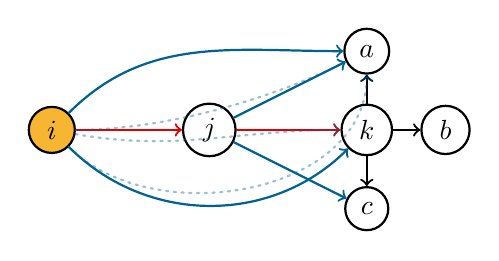
\begin{tikzpicture}[thick,line cap=round,scale=2]
	\tikzstyle{bai}=[circle,draw];
	\tikzstyle{hei}=[solid,circle,draw,fill=black,inner sep=.8pt];
	\node[bai,fill=myyellow] (i) at (0,0)           {$i$};
	\node[bai]               (j) at (1,0)           {$j$};
	\node[bai]               (k) at (2,0)           {$k$};
	\node[bai]               (a) at ($(k)+(0,0.5)$) {$a$};
	\node[bai]               (b) at ($(k)+(0.5,0)$) {$b$};
	\node[bai]               (c) at ($(k)-(0,0.5)$) {$c$};
	\draw[->] (k) -- (a);
	\draw[->] (k) -- (b);
	\draw[->] (k) -- (c);
	\draw[->,myred]  (j) -- (k);
	\draw[->,myblue] (j) -- (a);
	\draw[->,myblue] (j) -- (c);
	\draw[->,myred]  (i) -- (j);
	\draw[->,myblue] (i) to[out=45,in=180] (a);
	\draw[->,myblue] (i) to[out=-45,in=-135] (k);
	\draw[->,myblue,dotted,opacity=0.4] (i) .. controls ($(i)!2/3!(j)$) and ($(j)!1/3!(a)$) .. (a);
	\draw[->,myblue,dotted,opacity=0.4] (i) to[out=-10,in=180] (k);
	\draw[->,myblue,dotted,opacity=0.4] (i) to[out=-45,in=-90] (a);
\end{tikzpicture}

\end{document}
